\section{Motivating Example}
\label{sec:motivation}

% Context and Explanation of the example
To provide intuition about the problem, we present an exemplification of a mission execution by entities in a military context. Figure \ref{fig:2TeamExecution} illustrates a reconnaissance mission with some tasks randomly distributed requiring different types of sensors. In this mission, a team comprising four Unmanned Aerial Vehicles (UAVs) is interacting in a network configuration with a central leader, which is responsible only for providing instructions to its subordinates, e.g, distributing tasks among members. These interactions and network topology configure a specific C2 approach, named as \textit{Coordinated}~\citep{france2014}, based on the centralized distribution of information, patterns of interaction, and decision rights. The leader, marked in blue, guides the other team members to complete the tasks, i.e., obtain aerial images of particular points in the field, represented by red crosses.

% Highlighting the problem
The mission involves some natural risks that may lead to change in the conditions of execution. In our example, one member of the team, marked in red, fell due to some environmental change, such as an intense storm, causing damage to its motors. The loss of one entity, as depicted in Figure \ref{fig:2Drop}, can potentially decrease the quality of execution, in case that the task of the fallen drone remain unattended. With this in mind, a new plan is required and must consider the new tasks that originally belong to the fallen drone. One possibility to avoid the problem is to change the current C2 approach, i.e., change the network configuration and leaders. Furthermore, if the team changes to an unsuitable C2 approach or is not even capable of changing its C2 approach, both cases represent a lack of C2 Maneuver Agility. The absence of a strategy to increase C2 Maneuver Agility can cause the system to compromise the number of completed tasks at the end of execution. 

\begin{figure}
\centering
\fbox{
\begin{minipage}{.45\textwidth}
  \centering
  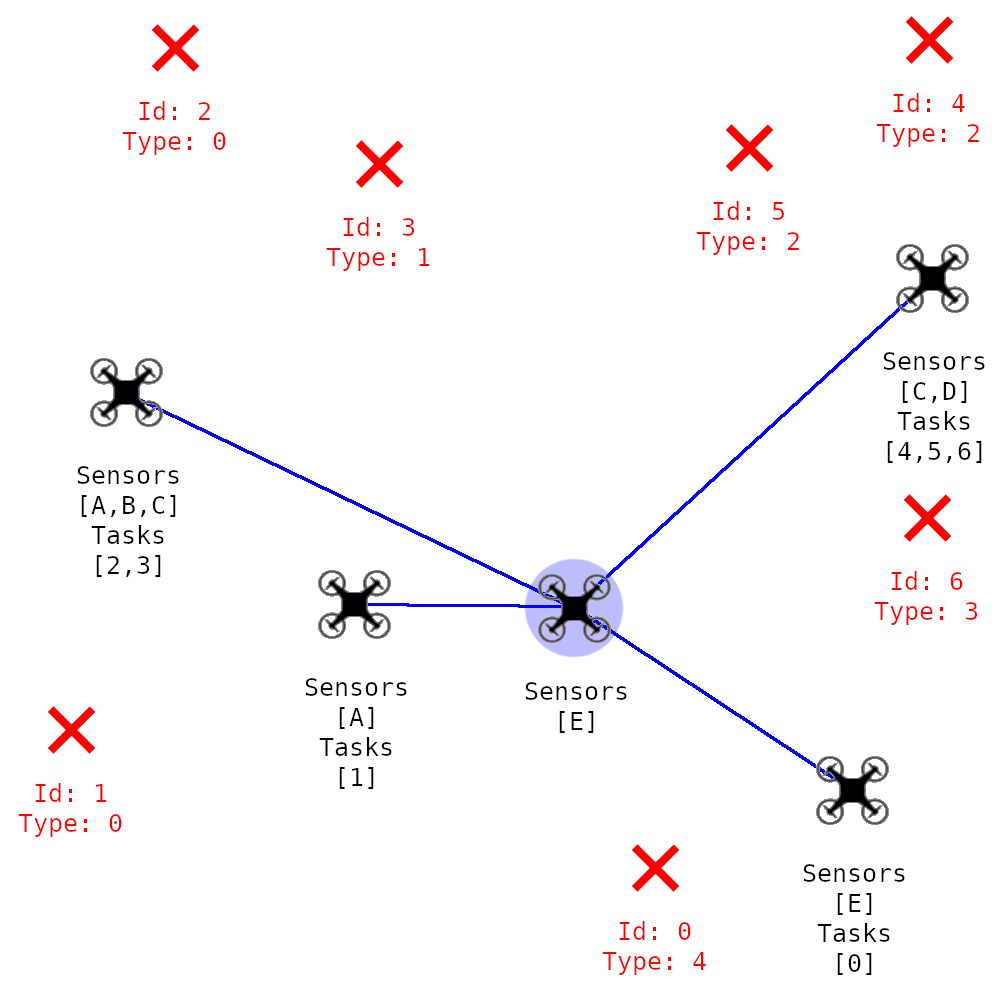
\includegraphics[width=0.95\linewidth]{figures/C2Drones1-V4.png}
  \captionof{figure}{Team of entities with the coordinator marked in blue}
  \label{fig:2TeamExecution}
\end{minipage}}%
\fbox{
\begin{minipage}{.45\textwidth}
  \centering
  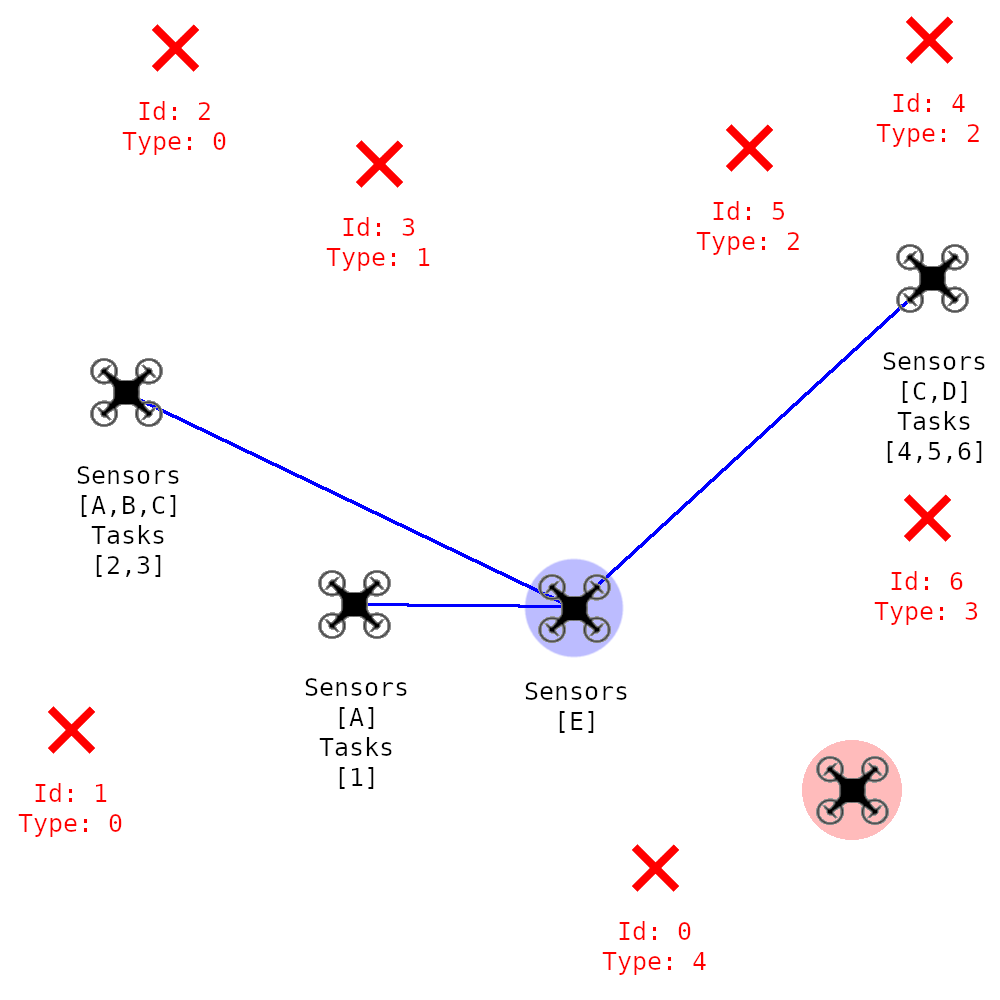
\includegraphics[width=0.95\linewidth]{figures/C2Drones2-V4.png}
  \captionof{figure}{Dynamic change with an UAV dropped marked in red}
  \label{fig:2Drop}
\end{minipage}}
\end{figure}

% Generalize the problem / Why is this not solved yet?
In general, some context changes, e.g., UAV failure, task addition, or sensor damage, must be considered during the mission planning. Indeed, no adaptation to the new context can impact quality results due to an incompatibility between entities and mission, or insufficient resources to complete the mission, or even the inability to meet minimum quality acceptance level. In other words, if there is limited C2 Maneuver Agility, the mission might be compromised.

Finally, Figure \ref{fig:3TeamExecutionAfterManuever} gives an example of a possible maneuvering strategy to maintain quality of execution. In this proposed example, immediately after the context change, the only member available for executing tasks type 4 is now offline. Moreover, the only member of the team capable of executing this new available task is the team's leader. Thus, after maneuvering to the \textit{Edge}~\citep{france2014} approach, the past leader can now participate in the execution of tasks, instead of only give orders to the team like in the previous strategy.

\begin{figure}[ht]
    \centering
    \fbox{
    \begin{minipage}{.45\textwidth}
  \centering
  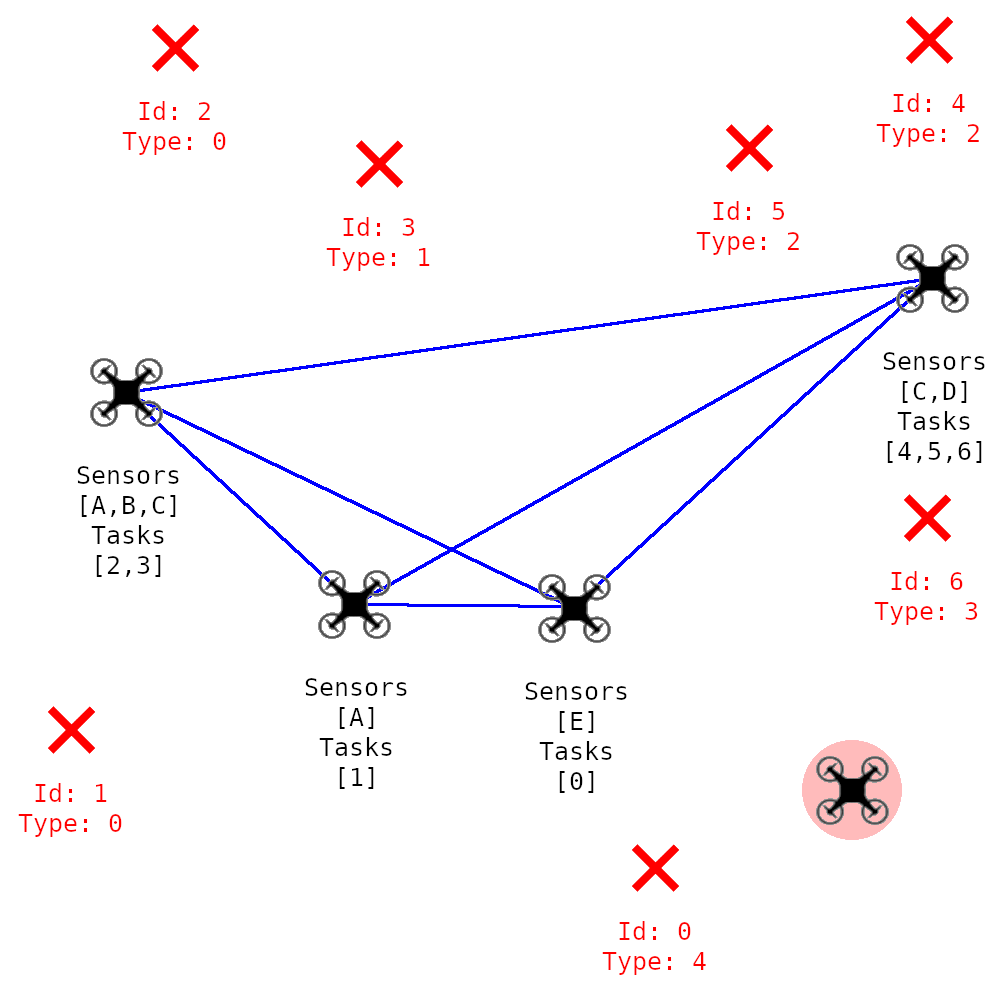
\includegraphics[width=0.95\linewidth]{figures/C2Drones3-V4.png}
  \captionof{figure}{Team executing tasks after changed C2 Approach}
  \label{fig:3TeamExecutionAfterManuever}
\end{minipage}}
\end{figure}